\documentclass{article} 
% \documentclass[12pt, a4paper]{article}

% Language setting
\usepackage[english]{babel}

% Set page size and margins
% Replace `letterpaper' with `a4paper' for UK/EU standard size
\usepackage[letterpaper,top=2cm,bottom=2cm,left=3cm,right=3cm,marginparwidth=1.75cm]{geometry}
\usepackage[style=apa, backend=biber]{biblatex} %use BibText
\addbibresource{references.bib}


% Useful packages
\usepackage{amsmath}
\usepackage{graphicx}
\usepackage[colorlinks=true, allcolors=blue]{hyperref}
% \usepackage{gb4e}
\usepackage{langsci-gb4e}


% \noautomath % solves the issue with gb4e incompatibility!
\usepackage[affil-it]{authblk} % For author affiliations. It provides better control over authors and affiliations. 
\usepackage{hyperref}          % For email links
\usepackage{setspace}  % for line spacing
% \usepackage{gb4e, cgloss} %for linguistics
\usepackage{langsci-gb4e}  %for glossing
\newcommand{\pref}[1]{(\ref{#1})} % for in-text example references

%%%%%%%%%%%%%%%TABLE%%%%%%%%%%%%%%%%%
\usepackage{booktabs} %%%%%%%%%%%%%%
%%%%%%%%%%%%%%%%%%%%%%%%%%%%%%%%%%%%


%authors affiliations
\author[1,*]{Matteo Radaelli}
\author[1]{Giosuè Baggio}

\affil[1]{\small Department of Language and Literature, Norwegian University of Science and Technology}
\affil[*]{\small Corresponding author: Matteo Radaelli, Department of Language and Literature, Norwegian University of Science and Technology, Postboks 8900, NO-7491 Trondheim, Norway; email: \href{mailto:matteo.radaelli@ntnu.no}{matteo.radaelli@ntnu.no}}

\title{Complement coercion with aspectual verbs is statistically infrequent in written Norwegian (?)}
\date{} %%leave it blank if you don't want to show the date
\begin{document}
\maketitle

\onehalfspacing

\begin{abstract}
%To be define in the end once RESULTS and DISCUSSION are completed.
% Combinations of an aspectual verb and an entity denoting complement (e.g., begin the book) have been often assumed to involve a mismatch between the verb’s requirements  (an event) and the complement’s denotation  (an entity; Pustejovsky 1991, 1995; Jackendoff 1997). Although this phenomenon has received considerable attention in English, its counterpart in Norwegian remains relatively unexplored. The objective of this study is to explore complement coercion with focus on Norwegian aspectual verbs in Norwegian with the intention to gain deeper insight into the structural variations of this phenomenon, with special attention to their syntactic patterns, variation in composition and frequency. 
% The corpus analysis was performed in four corpora, one web-based and three speechbased, taking into account the main aspectual verbs  (begynne ‘begin’, starte ‘start’, ende ‘end’, avslutte ‘end/conclude’, fortsette ‘continue’).
\end{abstract}
\noindent
\textbf{Keywords:} complement coercion, logical metonymy


%Theory: 
% from Hsu and Hsieh: In theframework of the Generative LExicon, a type coercion operation is defined as "a semantic operartion that converts an argument type to the type which is expected by a function, where it would otherwise result in a type error"
%From Hsu and Hsieh the complement coercion operation in the Generative Lexicon is not jut a theoretical construct, but it has also been empirically supported (e..g, Baggio et al., 2009, Delogu et al., 2010, Traxler et al.,2002, and Traxler et al. 2005) .(...) Te results of various experiments (eye-tracking exper, ErPs have shown that the processing cost i associated with the last stage, i.e., reconstructing an event reading for the NP complement. 
\section{Introduction}
Complement coercion refers to the phenomenon where an entity-denoting argument of a verb undergoes an interpretation of eventive type % JAckendoff 1997, Pustejovsky, 1991, 1995). 
An example is given in sentence in (1):

\begin{exe}
    \ex \begin{xlist}
        \ex John began the book.
        \ex John began reading/writing the book.
        \ex John began the football match.
    \end{xlist}
\end{exe}

\noindent In Sentence (1a), the verb \emph{begin} is supposed to be followed by a direct object as argument or a clause that specifies what is being started (an event), but here it is rather combined with an argument of entity-type (\emph{the book}), leaving the event implicit. The object as physical artifact per se cannot undergo an initialization phase, rather an activity done with the object is to be retrieved.  




% (e.g., nouns that contains sense of eventive type like concerts, matches, or reading a book)
% FROM ZARCONE; %2I follow here the broad distinction between "events" and "objects" (Casati and Varzi, 2010) exemplified
% by theWordNet ontology (Fellbaum, 1998), and refer with "entity" to the ontological class
% of "object" as opposed to "event". I will question the clear-cut distinction between (arguably
% metonymic) constructions combining event-selecting verbs with entity-denoting objects and (arguably
% non-metonymic) constructions combining them with event-denoting objects in the course
% of this dissertation.
The verb argument (\emph{the book}) is coerced into an event
Complement coercion occurs due to a 

% considerato interessante x via della violazione del principio di composizionalità e dalle numerose e recenti esperimenti psicolinguistici. 

% \section{Coercion in Norwegian}
\subsection{Frequency of Complement Coercion} % crossling.
Despite a rich presence of literature concerning complement coercion, there exists a noticeable gap in research concerning its occurrence frequency, mentioned only in a set of empirical and cross-linguistic researches. \textcite{shutova_logical_2009}  asserts from the analysis of the British National Corpus (BNC) made by \textcite{verspoor_conventionality-governed_1997} a high occurrence of logical metonymy in English, especially when combined with the aspectual verb \emph{finish}. In contrast to the claim made by the authors, the results of the corpus analysis present a different overview. Considering the whole corpus analysis of BNC\footnote{\textcite{verspoor_conventionality-governed_1997} analyzed also the Lancaster-Oslo-Bergen Corpus (LOB), but due to its small size},  
\textcite{verspoor_conventionality-governed_1997} could sample 4,470 of sentences that could contain the verb \emph{begin} combined with a noun phrase as argument but only 3.67\% (about 164 sentences) of these instances could be considered metonymic. A higher occurrence was instead found with sentences combined with the verb \emph{finish} followed by a NP, with 2,799 instances, when considering a sample of 11,072 candidate sentences. %bisogna dire che in effetti la possibilità di un'alta frequenza è possibile ma è solo ristretta ad un grupppo di verbi - e non mi stupisce che il verbo finire pare sia quello piu frequente. Vedi spalek Ma c'è anche da considrare che logical metonymy occorre anche in altri verbi e a quanto pare, se consideriamo il verbo begin non abbamo una distribuzione eequilibrata di istanze con logmeto.

\section{Methods}
\subsection{Corpora}
%tabelle e grafici prendi spunto su paper reporting verbs in court judgement-pdf

To provide a in-depth perspective on plausible candidates of coercion sentences and a comprehensive idea about how regular their occurrence is, we collected data from four distinct corpora, three of which are speech-corpora and one is text corpus. Consequently, by evaluating both corpora types, it allows us also to determine whether coercion is more frequent in spoken or written context. In this part of the section we enumerate and describe the employed 
corpora:

%noreference for the BB corpus! Just a link
The BigBrother Corpus is a speech corpus from the first season of the reality show Big Brother broadcast in 2001. The speakers are predominantly between the ages of 23-36 years, most from the eastern region of Norway. The corpus encompasses only 40 broadcast sessions out of 100 including a total of 440,300 tokens.

The CHILDES Norwegian Ringstad Corpus \parencite{larsen_byggeklossar_2014} is a contribution to the myltilingual collection of the Child Language Data Exchange System (CHILDES) database \parencite{macwhinney_childes_2000} and contains a subset of three speech corpora collected by three Norwegian children, all girls from age 1;10 to 2;8. Three children originate from teh Trondheim area, exhibiting acquisition and fluency in the local dialect. The Ringstad Corpus contains a total of 144 registrations with 2018 written transcriptions. We collected a sample of N=85 sentences where aspectual verbs occur.

Lastly, The NoTa-Oslo corpus \parencite{hagen_two_2014} is the last proposed corpus. It contains spontaneous speech from 166 speakers from the capital Oslo recorded from 2005-06. The group consists of individuals spanning from the age of 16 onwards including speakers from both low and higher education. The entire corpus consists of approximately 900,000 transcribed words.

The Norwegian Colossal Corpus (NCC) \parencite{kummervold_norwegian_2022} is currently considered the biggest text corpus available in the Norwegian language with more than 21M documents and 7B tokens. The corpus is a heterogeneous collection of sub-corpora coming from different sources,  including the National Library of Norway, an institution that aims to preserve and digitize hundreds of years of Norwegian texts from different domains such as newspapers, books, and journals. NCC also includes publicly available documents like for example juridical texts, government and general public reports, online newspapers and Wikipedia articles. A list of sub-corpora is presented in Table X in Appendix. Excluded from the data collection are scanned documents using OCR technology due to probable propagation of errors and noise that may cause issues in collecting and quantifying data. As \textcite{kummervold_norwegian_2022} mentioned, the digitized texts were collected at different points in time, and it should be noted that the quality of such texts may differ as a consequence of the advancements in OCR technology over the years.
% development of python script to heuristically select instances of logical metonymy. Consisting of four steps:

\subsection{Data Extraction}
% NCC_corpus_analysis_preprared.csv - original dataset using stanza.(exploration_NCC:train)
%exploration_NCC_train.ipynb 
%sentence_filtering.ipynb
%corpus preparation.ipynb
% nlp/corpus analyss/dataset_preparation.ipynb
%unify_two_datasets.ipynb unifies NCC_corpus_analysis_preprared_july_2023 and NCC_corpus_analysis_preprared
All corpora undergo the same processing for sentence detection which consist of basically three steps, such as (1) sentence extraction, (2) Sentence annotation, and qualitative and semantic evaluation of all candidate sentences. For this purpose, we developed a series of Python scripts to heuristically detect and filter candidate sentences for coercion in all corpora.
% Norwegian: bokmal or nynorsk?

%Extraction of those sentences which do not have an explicit VP complement.  
\paragraph{Sentence Extraction}
The first step of this corpus study involves the retrieval of all plausible sentences that encompass the aspectual verbs such as \textit{begynne}, \textit{starte}, \textit{fortsette}, \textit{avslutte}, and \textit{ende}. 
To accomplish this, we leverage Stanza Pipeline \parencite{qi_stanza_2020} and spaCy \parencite{honnibal_spacy_2017}, two natural language processing tools that offered robust solutions for tokenization, part-of-speech tagging, and dependency parsing. To optimize computational efficiency, especially when dealing with the considerable size of the NCC corpus, the extraction process was further divided into two distinct phases. Initially, for every article or raw text line in  case of speech corpora, a sentence tokenizer detected individual sentences. Subsequently, regular expression rules were applied to select only those sentences that contained the specified aspectual verbs. 
A drawback of this method is the higher recall in detection retrieving undesired sentences, such as instances including non-verbs (e.g., verbal nouns \textit{begynnelsen} 'the begin' instead of just the verb \textit{begynne}), but this ensured a much more scaled sample for the successive sentence filtering. Before being accepted, a language detector was employed for each sentence in order to ensure the selected sentences are written only in Bokmål, avoiding similar languages like Nynorsk and Danish\footnote{The NCC Corpus also incoroporates other (even non-scandinavian) languages, such as French, German, Spanish, etc. For further information see the \href{https://huggingface.co/datasets/NbAiLab/NCC}{HuggingFace Page}}.\\
The next step is fine-grain the research by exclusively selecting only canonical sentences which adhere the standard word order and syntactic rules in Norwegian, which in this case is SVO V2 \parencite[pp. 858-862]{faarlund_norsk_1997}. In order to find canonical sentences, NLP tools such ad part-of-speech (POS) tagger and dependency parser were employed. The primary goal was to pinpoint the aspectual verb as the root of the sentence, along its subject (nsubj). It was essential to maintain the correct word order, including only sentences where the subject precedes the main verb. The data obtained by dependency parsing is additionally filtered by selecting only instances considered as potential candidates for coercion. In line with previous remarks in Section X, the sole form of composition involves aspectual verbs combined either with NPs or PPs. Specifically, among prepositional phrases, the instance selection  will be done only on instances involving the prepositions \emph{på} and \emph{med}. 
%some text cleaning also performed

\paragraph{Sentence Annotation}
In order to refine the selection process, the second step involved a qualitative sentence annotation, identifying all candidate coercion sentences. This part was conducted by using four different classes:
% classified based on the head of the argument constituent. For the classification, four main classes were used   :
\begin{itemize}
    \item \textit{temp}: the constituent corresponds to a temporal denotation and therefore it is not considered an adjunct. 
    \item \textit{loc}: the constituent denotes a locative complement or adjuncts.  Bjørn Helge Riise startet på Norges midtbane da VM-kvalifiseringen ble innledet med tap borte mot Island fredag. Bjørn Helge Riise started in Norway's midfield as they opened their World Cup qualifying campaign with a loss away to Iceland on Friday.
    \item \textit{entity}: the constituent is identified as  an entity-denoting argument.
    \item \textit{event}: the constituent correspond to event-denoting argument.
\end{itemize}
As we can notice, coercion is only triggered by the 'entity' class whereas other categories do represent other semantic instances, thereby excluding them from being considered as candidates for our analysis. The purpose of using four different classes is not only gaining a deeper understanding of complement coercion but also to obtain a better insight of the role of aspectual verbs in Norwegian in terms of compositionality. Since all the selected corpora were basically raw text with no particular semantic information, the entire analysis will be carried out manually. 


% queste classi sono 

%selection based on semantic type
\paragraph{Selection of entity-denoting arguments.} The target sentences must be selected based on the semantic type of the argument. As we already know, complement coercion occurs with the co-composition of an aspectual verb and an argument of entity type. For that reason, the last step of data extraction implies a subsampling of sentences with entity-denoting argument and further semantic analysis is done with the objective to identify cases of complement coercion. 
%problem with definition of entity
%selection of transitive sentences wirth animated subjects 
One challenge encountered while working on entity classification was the difficulty in establishing clear guidelines for defining entities that could cause complement coercion, since there is not a precise universal definition for what constitutes an entity. In the analysis mentioned in \textcite{rud_covert_2011} and \textcite{zarcone_logical_2012}, for example, the author opted for sampling artifact objects, in the sense of physical and tangible %and digital?
items(?), excluding entities with ambiguous denotation with no clear distinction between entity and event reading. % e.g., cigarettes, letters
%incorrectly extracted sentences removed, maybe due to some error. 
% Metaphorical uses were excluded. 
\textcite{verspoor_conventionality-governed_1997}, on the other hand, does not explicitly specify any
entity selection for her research. The intention of the author was collecting sentences with aspectual verbs and non-VP constituents that could be potentially metonymic, only excluding some cases where the sentences were events, entailed temporal denotation.
However, relying solely on artifacts can be limited, since also some more abstract nouns can also interpolate an event. An example can be the noun 'story', since, due to its polysemy, it can also refer to facts that can typically be read, written or told. % mention that a list will be shown somewhere.

A particular attention should also be given to instances where the verb argument may consist of an entity  but it cannot be considered coercive:
\begin{itemize}
    \item Aspectual verbs such as \emph{begynne} and \emph{avslutte} include argument constructions V + \mbox{\emph{V + NP + med}} that impose a different interpretation of the action compared to coercive and metonymic constructions, as the action itself refers to a broader activity. %Verspoor 1997b
    For that reason, such constructions cannot be included as candidate:

        \ea %NCC
        \gll Vi avslutter derfor rapporten med et kapittel 10 som beskriver Finland spesielt.\\
             We finish therefore report-the with a chapter 10 that describes Finland especially.\\
        \glt ‘We therefore conclude the report with a chapter 10 that describes Finland in particular.’
        \z

    \item In some cases, aspectual verbs also exhibit polysemy, including other senses than the conventional meaning. The verb \emph{begynne}, for example, typically denotes initiation, but it may also be employed with the sense of \emph{found} or \emph{join}, notably within corporate establishments, newspapers, political parties, music bands, etc.:

        \ea %NCC
        \gll Torgrim Melhuus startet bedriften sammen med søsteren Trine Melhuus i 2002.\\
            Torgrim Melhuus started company-the together with sister Trine Melhus in 2022.\\
        \glt ‘Torgrim Melhuus started the company with his sister Trine Melhuus in 2002.’
        \z
        
% Marie Lundström begynte på Sveriges radio i 1995 og har laget ulike litteraturprogram i radio, blant annet ''Lundströms bokradio'' i P1.


    \item A particular complement highlighted by \textcite{verspoor_conventionality-governed_1997} referred to as \emph{event-object} is also to take into account. This is attributed to the inherent flexibility of the NP to be used as both event and entity, allowing for metonymically interpretations.  Examples that fall under the umbrella of event-object instances encompass nouns such as `lessons', `course', `speech', etc.: % check here in NCC.

        \ea \label{lesson_example} %NCC
        \gll  Sindre begynte på svømmekurs da han var fem år.\\
            Sindre began on {swimming-course} when he was five years.\\
        \glt ‘Sindre started (taking) swimming lessons when he was five years old.’
        \z
    \item[] For instance, the Sentence~\pref{lesson_example}, the NP \emph{svømmekurs} (`swimming lessons') % correct the formatting?
can serve as event-object, enabling an interpretative interpolation with eventive nature of taking swimming lessons.
Conversely, in the scenario where the aforementioned lessons are intended as 'giving lessons', the whole argument should be considered of an eventive type, and therefore not considerable as coercion candidate. Given the antecedent conditions, only sentences with entity-denoting arguments will be integrated in the study, with the event-denoting nouns being excluded.
% PAROLE CO EPROGETTO ENTRANO NEL PROBLEMA DI COMEI INTERPRETARLI


        \end{itemize}

%temporal objects -discarded  -something with temporal extent. no type coercion is necessary.


%     \ea 
%     \gll Vi starter kapitlet med en presentasjon av teoretiske tilnærminger til iverksettingsbegrepet.\\
    
% We start chapter-the with a presentation of theoretical approaches to the-concept-of-implementation.\\
%     \glt ‘We start the chapter with a presentation of theoretical approaches to the concept of implementation.’
%     \z




% \begin{exe}
%     \ex 
%     \gll hello \\
%     \glt ca
% \end{exe}



% This is another gloss\\
% \glt `This is a translation.'\hfill (Language information)
% \end{exe}


%The concept of aspectual verbs in linguistics relates to verbs that convey information about the temporal structure of an action, whether it's ongoing, completed, repeated, etc. Aspectual verbs can be influenced by the syntactic structure of a sentence, and they play a role in shaping the temporal interpretation of an event.

% Vi starter derfor kapittelet med å undersøke om elever og lærere etter tre år med arbeidslivsfaget opplever at faget har vært praktisk.
% Vi avslutter derfor rapporten med et kapittel 10 som beskriver Finland spesielt.
% Et norsk firma med hovedkontor i Halden startet privat barnehage ved Svinesund, på svensk side fordi de har så mange svenske ansatte.
%duplicates are also excluded


 
%At the end of this phase I had a large collection of sentences which were potentially metonymic, as each sentence contained an aspectual verb followed by a non-VP element.

%second phase: Resolution of underspecification(morphosyntactic information to distinguish subject and objects)  and  identification of the collected sentences were actually metonymic. neither of the corpora contains any kind of semantic tagging, much of this work had to be done by hand. Following cases were eliminated:
%Sentences in which the aspectual verb appears as part of a larger phrase which seems to impose different interpretation constraints on the phrase that on the metonymic constructions. These include begin X with.
%Sentences  containing different senses of the aspectual verbs: found, initiate: she bagen a smile, began a ritual, habit, sense of finish meaning of use up (es. finish toilet paper. 
%Sentences In which the noun phrase complement is eventive, that is directly expressing an event such that no metonymic construction is necessary. This case includes deverbal nouns (begin a look, the cut, inspection) also other instances begin the  game,begin a diet. In these cases, no type coercion is necessary to satisfy the requirements of the aspectual vrbs, 
%Sentences in which the noun phrase complement is temporal, referring to something with temporal extent (begin a relationship), begin the first term of school) + pinango idea 

%Sentences containing event-objects as compleemtns: dual nature NPs which seem to have a natural interpretation as an event, but which can also be referred to as an object. these can be either interpreted ad events directly or, with certain restrictions, metonymically on an object interpretation. Only the metonymic uses are included in the analysis: john began the speech/lesson (giving) - classified as eventing
%JOhn began the speech/lesson (writing) metonymic ?????ma perche?

%incorrectly extrcted sentences were removed, Some errors were due to pasing errors insentences structure or in the subject annotation. (problems also by text itself) 
%Zarcone: many nouns were ambiguous between an entity and an event reading, breakfast, report, painting. unless the context clearly suggested an artifact reading, these sentences were omitted. The proportion of discarded sentences for the abobe mentioned reasons was etbetween 30% and 50%. The selected meto sentences were then analyzed and annotated with CE paraphrases and the QRs for their objects were determined. 



%Third phase: read through each of the metonymic sentences in context in order to determine the interpretation intended by the speaker/author. 
% spiega come sono stati classificati. 
% if only little context was available, finding a suitable paraphrase was often not easy. Short sentences impossible to choose among several possible alternatives. 
% PP attachment - controlla text. PP in 10 mit dem Ball is an oblique argument of spielen also in the paraphrase. 
% transparent nouns: in cases of trnasparent nouns such as cup of coffee, (Fillmore, Baker, & Sato, 2002) the content was regarded as the real object of interest (coffee), instead of the direct object of the verb (cup)

%%% The whole procecude was repreated to find meto instances of the phrase begin on. 



%%%% Verspoor: Most analyses of logmeto have two limitations.  FOcus on english. Few studies compare English with French other languages are hardly ever analysed (Horacek 1996 and a very recent paper by Ru¨ d and Zarcone (2011) being notable exceptions). Only four studies on logmeto that use examples from corpora (Briscoe et al. 1990, Lapata and Lascarides 2003, Ru¨ d und Zarcone 2011, Verspoor 1997a). Briscoe, Copestake and Boguraev did a very small corpus study of a total of 235 examples and Lapata and Lascarides use real data only to check automatic predictions on the interpretation of logical metonymies. Verspoor exhaustively analysed corpus examples of logical metonymy with the verbs begin and finish. Ru¨ d and Zarcone examined the German equivalents anfangen (mit) (‘to begin’), aufho¨ren (mit) (‘to stop’), beginnen (mit) (‘to begin’), beenden (‘to finish’) and genießen (‘to enjoy’) in combination with artefacts as direct objects.
%%% Menzionare il lavoro di Verspoor, Sweep e quello cinese. Sweep extends previous research by comparing the behavior of log meto in Dutch, German, and English.

%%%Different verbs allowing lofgicalmetonymy are very different in their structurees. German verbs such as beginnen and enden mit or Dtucg beginnen and eindigen cannot only be used transitive, but alos intransitive, in such cases the event that is started or finished occurs as the subject.  Such constructions are not posible with German geniessen and beendedn owr Dutch beeindigen andgenieten van
%%%% BEGIN ON: Verspoor: begin on + NP generally seems to serve as syntactic marker for pragmatic interpretation. It indicates only that something is being done with the NP object, leaving a more specific interpretation to be established using contextual information. It does not need to look to the qualia structure for a default inerpretation, as context will provide the interpretation.
% JEspen: Whereas Verspoor found that only a limited number of specific nominal categories are used metonymically with English begin, Dutch and German appear to be to be even more restrictive in selecting concrete direct objects.

%%% Jespen: In germman almos all meto dir objrefer to stories or text, all with agentive interpretation, begin a piece of music or beginning a store company. <- in questo caso lei inserisce begin company come metonimia allora? Metonimia logica potrebbe accettare anche quersto tipi di costruzioni? Se si allora non si spiega il motivo per cui Verspoor begin a company (ovvero espressioni che hanno un altro tipo di interpretazioni) vengano accettate.
%% nl beginnen np shows results similar  to German, with same categoeries. Telic interpretations are very marginal (es. reading book )
%%% nl beginnen met: started action is the first in a series of comparable actions. This means that is is a sub-part of a larger coherent action or the start of a repeated action. The action can be left implicit. 

%%%% beginnen NP met pag 8 - considered metonymycal. THe combination of  DIRobj and prepositional object with beginnen corresponds to the interpretation of a sub-action V belonging to a more general action W:The prepositional obj specifies the furst sub-action V of more general event or action, which can be expressed as a dirobh (or also passive subj). explains why more concrete complements and more context-dependend eventive interpretations are used as met-ibjects. The inference to the implied acion V is easierxk the started (implicit) med-event is related to another action (V or W) which is in all probability known in context. In this way the prepositional object maked it easier to interpret the combination with a concrete noun as compared to the interpretation of a direct object denoting a conrete entity. The event V tgat is needed for a full interpretation must be some action related to other actions (the repetition of V or more general action W)

%%%% beginnen aan must have specific semantic properties as compared to beginnen NP xk combinations of concrete nouns only occur with beginnen aan. (beginnen with sandwiches and other type of food). In most cases telic interpretations. OTher examples with aan,  beginnen with concrete objects and strongly context-dependent metonymy! Whereas beginnen + NP needs to be combined with an event-denoting dirobj and can occasionally be used with certain thing-denoting words that are closely associated with a specific event, beginnen aan can be used with all kinfs of nouns and  pronouns. <<<- simile in alcuni casi con Verspoor begin on? 
%%% prep aan marker of log meto  not possible to identify as marker of logmet. there is some independent aspect of beginnen aan that makes logical metonymy easier to undertsand. Honselaar, mentions that beginnn ann alwaysn strongly brings into mind the idea of an event,  a projection of an event. with aan could be together with an event or a concrete entity related to an event. beginnen aan brings an event as a completed whole into mind. Honserlaar suggests that the aan-complement evokes the idea of an event which the subject started in a stronger way that beginnen + direct object does. it is this projection of ane ecent.  THis underlying semantic is reflected in the syntactic requirements of beginnen aan:In contrast to beginnen + DirObj beginnen aan can only be combined with verbal nominalizations and not with infinitives. 

% Marie begon het boek (te lezen)
% Mary began the book (to read-INF)
% ‘Mary began (to read) the book’
% (24) Marie begon met het boek (te lezen)11 / met (het lezen van) het boek
% Mary began with the book (to read- INF) / with (the read- SUBST of) the book
% ‘Mary began with (reading) the book / with (the reading of) the book’
% (25) Marie begon aan het boek (*te lezen) / aan (het lezen van) het boek
% Mary began on the book (*to read- INF) / on (the read-SUBST of) the book
% ‘Mary began on (*reading) the book / on (the reading of) the book’
% 128 Josefien Sweep
% Downloaded from http://ijl.oxfordjournals.org/ at University Of British Columbia Library on July 11, 2015

% HOW IS IT IN NOR?


%%% verbal nominalization  - it conceptualizes the event as a kinf of thing. The syntactic requirements of beginnen aan imply tht it is not that some event in general is required, as required in beginnen + NP., but rather that some abstract event as a king of think-like entity is evoke. The meaning aspect is in line with HOnselaar's analysis that in the case of beginnen an we think of the event as a projected enityt, which is not the case for beginnen met or with NP. SEmantic difference is reflected in the syntactic form of the different types of objects.  As consequence the syntactic requirements of beginnen aan directly indicate the meto to a hearer, if the verb is combined with a word that refer to a concrete enrtity. Whereas hij begint (met) een boek couls still be followoed by a verb . Not pox with begint aan een boek.
% both aan and methave inherent properties nothing to do with logmet, which explain why prep objs are more often used in logmeto constructions.  Both suitable with nouns, beginnen met als o used in constructions with two nouns to express that event start with another event.  begunnen aan, activity is already brought into mind and the syntactic form directly indicates that the combination with a noun referring to a concrete entity has to be interpreted metonymycally. In the case of beginnen met with agentive subject the specific meaning aspect of prep object helps us to undertsand the intended actibity: the event that is needed for a full interpretation must be some action related to other actions in context. 
%%% Marie begynte med å lese boken. la preposiione med non introduce alcun fenomeno di metonimia logica. Invece con la preposizione paa si puø notare questa cosa. Tanto che una costruzione sintattica infinitiva non e' possibile. PAre andare nella stessa direzione di Jespeer. MA QUESTO va bene? HO visto che su google begynne på å, esistono alcune espressioni ma sono pochissimi!!!! potrebbe andare bene? Mi pare di no!  la preposizione på potrebbe indicare un+espressione di volonta' di iniziare qualcosa mentre NP no. Il fatto che ci sia med lqa costruzione sopra citata pare ancora valida inoltre indica anche quella una non intenzione ,a si vuole di piu indicare una volonta nell+iniziare una serie di cose partendo con quella che si esprime come argomento del verbo.
\section{Results}
To begin with, a comprehensive distribution of the aspectual verbs in the NCC corpus is shown in Table~\ref{frequency_aspectual_verbs}, specifically highlighting the absolute frequency of the sentences containing the aspectual verbs as main verbs that satisfies the criteria mentioned in the previous section. The relative frequency (Rel. Freq,) indicated from the data refers to the proportion of occurrences of the verbs relative to all the occurrences of the aspectual verbs in the sample. 
\begin{table}[h!]
\begin{center}    
\caption{Frequency of the aspectual verbs in the NCC corpus. }
\label{frequency_aspectual_verbs}
\begin{tabular}{lcr}
\toprule\toprule
Verb &    Freq. (raw) &  Rel. Freq.\\
\hline
 starte &  107285 &               0.434387  \\
begynne &   65186 &               0.263932  \\
 fortsette &   44762 &               0.181237 \\
avslutte &   22157 &               0.089712  \\
 ende &    7590 &               0.030731  \\
  \hline
 TOTAL & 246980\\
\bottomrule
\end{tabular}
\end{center}

\end{table}

\noindent The data indicates a noticeable difference in occurrences between verbs. The data reveal that the initiation verbs occur more often than the other verbs: the verb \emph{starte} covers 43\% of the total sample, indicating that it is the most frequent aspectual verb in the NCC corpus among the listed verbs. The verb \emph{begynne}, while not as frequent as the previous verbs, shows a considerable presence in the corpus, with 26\% of relative frequency. Particularly interesting, instead, is the low frequency of the verb \emph{ende} with less than 7600 instances detected and covering only 3\% of the entire sample. In the next section we will go deep into the analysis divided by verb. The results presented as follows: %...section x you do this ...


%MANCA TUTTA LA PARTE RELATIVA ALLA SUDDIVISIONE DEI POS TAGS

%want present a quantitative and qualitative results
%. Since the corpora investigated vary in size, the normalized frequency per 100,000 words is given in the columns headed (Frequency per 100K words). Normalized frequency reports frequency against a common base of normalization as a proportion of each corpus, (see e.g McEnery and Hardie 2012, 49). 


%include frequency divided by verbs. 
\subsection{Coercion and logical metonymy with initiation verbs}
The preliminary focus of this corpus analysis encompasses the verbs of initiation, such as \emph{begynne} and \emph{starte}. In this subsection, we will discuss the syntactic composition of these two verbs, trying to understand what words follow the predicates and how they are distributed. After a quantitative analysis, we will gain insight into the possible entities identifiable in the corpus sample by semantically analyze the sentences and their plausible induction to coercion.

To begin with, Table X illustrates a quantitative analysis of word frequencies based on POS tag in the context of both initiation verbs. For practical reasons, we do not present every single tag in the table, and minor tags are therefore merged into the category "OTHER". Analyzing  the verb \emph{begynne}, the particle \emph{å} (PART) is one of the more frequent type of words found after the verb, with 24,718 occurrencies representing 37\% of the entire sample. Prepositions (ADP) rank as the next prevalent POS, with a frequency of 20,823 occurrences (31\% of relative frequency). Less frequently observed phenomena include noun phrases with minor occurrences of nouns (NOUN), with 8\% of relative frequency and determiners (DET) comprising only 2\%. 
A slightly different trend can be found in the results of the verb \emph{starte}. Prepositions seem to be the more frequent syntactic category found after the verb, with 57,613 instances covering approximatively 53\% of the entire sample, followed by nouns with 23,531 frequencies (21\% of relative frequncy). Interestingly, the particle \emph{å} assumes here a less prominent role in comparison to its counterpart, with only 843 instances found.

%ADD SCONJ?
Comparing the distribution analysis of both verbs we can infer that there is a compositional variability according to the verb used with some divergences and some similarities. Figure~\ref{fig:barplot_pos} compare the frequency of POS between verbs. Notably, Norwegian speakers would apparently tend to introduce mostly infinitive clauses when combined with the predicate \emph{begynne}. The verb \emph{starte}, on the other hand, seems to avoid these compositions, preferring other alternatives such as noun phrases, which are more consistent in the sample. Very interesting is instead a high presence of prepositions in both verbs, which can make good candidate for composing complement coercion. 

%table distribution of prepositions of begynne
% \begin{table}[!]
%     \centering
%     \begin{tabular}{lrrrr}
%         \toprule
%         \midrule
%      Prep.   & Freq. & REL.FREQ. Prep & REL.FREQ. Verb \\
%      \hline
%      i       & 8162 & 0.391970 & 0.125211 \\
%      med     & 5774 & 0.277290 & 0.088577 \\
%      på      & 2886 & 0.138597 & 0.044273 \\
%      for     & 821 & 0.039428 & 0.012595 \\
%      etter   & 743 & 0.035682 & 0.011398 \\
%      ved     & 734 & 0.035249 & 0.011260 \\
%      før     & 228 & 0.010949 & 0.003498 \\
%      fra     & 150 & 0.007204 & 0.002301 \\
%      under   & 135 & 0.006483 & 0.002071 \\
%      omkring & 134 & 0.006435 & 0.002056 \\     
                    
%         \bottomrule
%     \end{tabular}
%     \caption{Table Caption Here}
%     \label{tab:prep_begynne}
% \end{table}

As our goal is to explore the key elements that may trigger complement coercion, we proceed with an in-depth exploration of preposition distribution, in particular the prepositions \emph{på} and \emph{med}. In order to do this, we will restrict the sample to include only initiation verbs followed by prepositions.
Table~\ref{tab:prep_begynne} provides the absolute frequency of sentences with the 10 most frequent prepositions that follow the verbs \emph{begynne} and \emph{starte}. 
% In addition, the table provides the relative frequency within the subsample of only prepositions for each verb, and a further relative frequency based solely on the verb frequency.
In addition, the table provides the relative frequency normalized by the total amount of canonical sentences that occur with the corresponding verbs. Comparing the distribution across predicates, we can notice consistent results. 
The preposition \emph{med} and \emph{på} appear to be the most frequent among others. The former preposition is found in 5,774 instances in begynne, and 10,817 instances with \emph{starte}, with a relative frequency of only 8\% and 10\% respectively. The latter preposition, instead, is less frequent, with 2,866 with \emph{begynne} and 4,933 with \emph{starte}, with only 4.5\% of relative frequency for both verbs. This analysis highlights two important aspects related to the word distributions combined with initiation verbs. Firstly, the preposition that may arise complement coercion seem to be consistent across verbs, demonstrating similar proportions in occurrence between both verbs. Secondly, their occurrence appears to be quite infrequent, covering a low portion of the corpus.   


%paritre a descrivere la differenza in preposizioni paa e med. 

% 1. **Prepositions (ADP):**
%    - With an absolute frequency of 78,436, adpositions (prepositions) are quite prevalent in the dataset.
%    - This suggests that the verbs "starte" and "begynne" are commonly associated with specific prepositions, indicating a strong syntactic relationship with other elements in a sentence.

% 2. **Nouns (NOUN):**
%    - Nouns have a substantial absolute frequency of 29,280 occurrences.
%    - The high frequency of nouns implies that these verbs are frequently used in contexts where concrete objects, actions, or entities are being initiated or commenced.

% 3. **Pronouns (PRON):**
%    - Pronouns occur 8,379 times, indicating that references to specific individuals or entities are common in the proximity of these verbs.
%    - This could suggest that the verbs "starte" and "begynne" often involve actions or events initiated by or involving specific actors or entities.

% 4. **Particles (PART):**
%    - The absolute frequency of particles is 25,581.
%    - The high occurrence of particles suggests that there might be nuanced or specific meanings associated with the use of these verbs, and particles play a significant role in expressing these nuances.

% 5. **Subordinating Conjunctions (SCONJ):**
%    - Subordinating conjunctions have an absolute frequency of 14,945.
%    - This indicates that the context of "starte" and "begynne" often involves complex sentence structures, where one action or event is subordinated to another.

% In summary, the high absolute frequencies of adpositions, nouns, pronouns, particles, and subordinating conjunctions suggest that the verbs "starte" and "begynne" are versatile and are used in diverse syntactic and semantic contexts. Researchers could further investigate specific prepositional phrases, noun phrases, and syntactic structures to gain a more nuanced understanding of how these verbs are employed in Norwegian discourse.


%inserire anche la tabella con le frequenze
\begin{figure}[htp]
    \centering
    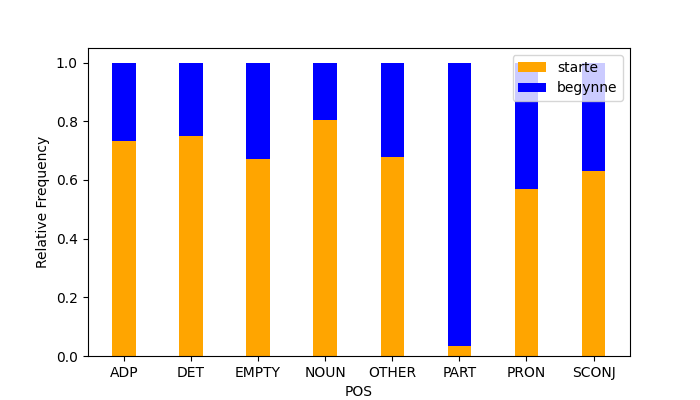
\includegraphics[width=10cm]{pics/barplot_pos.png}
    \caption{Comparison of frequency of different words based on their POS between the verbs \emph{begynne} and \emph{starte}.}
    \label{fig:barplot_pos}
\end{figure}

\subsection{Sentences with prepositional phrases}
%med: pox avere complemento di compagnia.
%idea presa da uso di parlanti.
As previously mentioned the combination of initiation verbs with prepositional phrases may be the key elements for triggering complement coercion, more precisely when the phrase is introduced by the prepositions \emph{på} and \emph{med}. %cit NOT FOUND
For that reason, the next step of our research is a semantic analysis of sentences combined with aspectual verbs and the aforementioned prepositions. Additionally, it is important to point out that complement coercion occurs only in cases where the sentence include subjects of agentive type. 
\begin{table}[!]
    \centering
    \begin{tabular}{lrrrr}
        \toprule
        & \multicolumn{2}{c}{\textbf{Begynne}} & \multicolumn{2}{c}{\textbf{Starte}} \\
        \cmidrule(lr){2-3} \cmidrule(lr){4-5}
        \textbf{Type Subj.} & \textbf{på} & \textbf{med} & \textbf{på} & \textbf{med} \\
        \midrule
        non-agentive &   988(0.05/ 0.02) & 3451(0.17/0.05) & 2157	(0.037/0.02) & 7510(0.13/0.07)\\
        agentive      &  1154(0.06/0.02) & 1366(0.07/0.02)  & 612(0.01/0.005) &  1911(0.03/0.018) \\
        \bottomrule
    \end{tabular}
    \caption{Table Caption Here}
    \label{tab:initiation_verbs_agentive_no_agentive}
\end{table}
% 0 & Preposition & agentive? & Sentence & REL.FREQ_ADP & REL.FREQ_VERB \\
% 7 & på & agentive & 1154 & 0.055419 & 0.017703 \\
% 9 & på & no agentive & 988 & 0.047448 & 0.015157 \\
% 0 & med &  & 933 & 0.044806 & 0.014313 \\
% 5 & på &  & 646 & 0.031023 & 0.009910 \\
% 10 & på & not necessary & 81 & 0.003890 & 0.001243 \\
% 3 & med & no & 18 & 0.000864 & 0.000276 \\
% 8 & på & no & 14 & 0.000672 & 0.000215 \\
% 1 & med & ? & 2 & 0.000096 & 0.000031 \\
% 6 & på &  no & 1 & 0.000048 & 0.000015 \\
% From this distribution, it can be inferred that a significant portion of instances involving verbs of initiation involves subjects without clearly specified agents, emphasizing a more passive or indeterminate initiation process. Additionally, the presence of agentive subjects, though less frequent, suggests that there is a noteworthy subset of instances where the initiation is explicitly attributed to an agent or initiator. This nuanced analysis provides valuable insights into the syntactic patterns associated with verbs of initiation and contributes to a deeper understanding of the linguistic structures governing such constructions.
Table~\ref{tab:initiation_verbs_agentive_no_agentive} shows the frequency distribution of subjects in sentences that include initiation verbs as predicate. The values are divided based on the subject type ("agentive" and "non-agentive") and the preposition "på and "med" that follow the verb. Furthermore, the table provides the relative frequencies normalized by the total amount of canonical sentences occurring with the corresponding verbs.
The frequency of sentences containing agentive subjects is relatively low, with 1154 and 1366 annotated instances with the verb followed by the prepositions "på" and "med" respectively in case of the verb \emph{begynne} as predicate, and 612 and 1911 for \emph{starte}, with a relative frequency score of equal or even less than 2\%.
% This trend suggests that the occurrence of sentences with agentive subjects is particularly infrequent, and going deeper into the semantic analysis of sentences with agentive subjects the situation is not better. 
Table~\ref{tab:semantic_initiation_verbs_adp} and XX show the distribution of semantically annotated sentences with initiation verbs occurring with agentive subjects and prepositional phrases introduced by the prepositions på and med respectively. From the results, it is clear that one of the primary use of prepositional phrases is to introduce arguments of eventive type, with 241 instances with \emph{begynne} and 84 with \emph{starte}. Furthermore, the preposition \emph{på}, due to its nature to mark locative adjucts (Tungseth, 2008)
% Tungseth, Mai Ellin (2008). Verbal Prepositions and Argument Structure: Path, Place and Possession in Norwegian, John Benjamins Publishing Company.
, includes 168 and 282 occurrences. 

\begin{table}[]
    \centering
    \begin{tabular}{lrrrr}
    labels & freqs\_begynne & REL.FREQ\_VERB\_x & freqs\_starte & REL.FREQ\_VERB\_y \\
    entity & 170 & 0.002608 & 84 & 0.000783 \\
    entity? & 2 & 0.000031 & nan & nan \\
    event & 241 & 0.003697 & 160 & 0.001491 \\
    loc & 168 & 0.002577 & 282 & 0.002629 \\
    no & 17 & 0.000261 & 5 & 0.000047 \\
    other & 39 & 0.000598 & 34 & 0.000317 \\
    pron & 9 & 0.000138 & 1 & 0.000009 \\
    skole & 469 & 0.007195 & 15 & 0.000140 \\
    temp & 39 & 0.000598 & 29 & 0.000270 \\
    ? & nan & nan & 2 & 0.000019 \\
    \end{tabular}
    \caption{begynne,starte,på}
    \label{tab:semantic_initiation_verbs_adp}
\end{table}
%entity-denoting arguments
In terms of  sentence frequency including entity-denoting arguments, the table shows a relatively small group of instances, with 170 identified sentences with the verb \emph{begynne} and 84 with \emph{starte}. Among them only a restricted amount of sentences could be plausible candidates for complement coercion. The verb \emph{begynne} presents 128 instances of coercion, while \emph{starte} includes only 55 sentences. 
The types of entities found ranges that span from pure artifacts to less concrete objects, with books and text being among the most frequent encountered. 


    \ea \label{sent:initiation_paa_1} %NCC

    \gll Dostojevskij begynte på "Forbrytelse og Straff" sommeren 1865.\\
         Dostoevsky   begynte on "Crime and Punishment" summer 1865.\\
    \glt ‘Dostoevsky began "Crime and Punishment" in the summer of 1865.’
    \z




%CONTINUA ORA A SPIEGARE QUALI SONO I FENMENI DI COERCION TROVTI CON PAA
%check sentences with class agentive? 
%check sentences with class entity? how to treat them? 





\subsubsection{The case of skole}
%%%%WITH PAA: some of words that can be considered something like entities are difficult to consider them as coercion.  
%skole, universitet
%attend (seminar)= = attend  seminar but in Norwegian we cannot interpret it as begin joining the seminar.  For that reason considered as eventive? - - check join: %begynne paa jotul (join?)= start working at jotul. how to classify?  - Some sentences: begynne på byggfag - begynne å studere byggfag seems ok.
% one case with project: begynne på prosjekter - not entity but series of events. 






Particular attention should also be given to the term "skole" and its synonyms ("universitet", "ungsomskole", etc.):
        \ea \label{initiation_skole} %NCC

        \gll En del gutter begynte på universitet i en alder av 14 år.\\
             One part boys began at university in an age of 14 years.\\
        \glt ‘Some boys began university at the age of 14.’
        \z
The occurrence frequency of such sentences is particularly high, especially when introduced by \emph{begynne}, with 469 sentences, whereas with the verb \emph{starte} is in comparison infrequent, appearing only 15 times. 
The combination of the aspectual verb and the phrase "på universitet", even though the university transcends a spacial designation, does not imply only a locative adjunct, but it is also considered an institution, suggesting the act of commencing a period of study course at the university. For that reason, the question that may arise is whether to treat this combination as an argument of eventive type, in the sense of a range of time when a series of sub-events may occur, or classify the word "universitet" as a special case of complement coercion, considering the term as a proper entity.
%il fatto che è molto presente questa costruzione ci fa pensare che viene utilizzato in maniera idiosincratica? 
%two problematics with considereing it as CC phenomenon: traditionally interepretation of entities by changing the  syntactic type of constituent: beginne på boken (PP) - begynne å lese boken (NP) -  beginne på universitet (PP)  - begynne å studere på universitet (PP). Semantically universitet, if finding an interpretation, we do convert the object into a locative. 
%cosa differente le espressioni per indicare iniziare il lavoro da qualche parte. begynne på Ikea - in ita iniziare da Ikea - non sempre necessario un'interpretazione completa.  





\subsubsection{Sentences with direct objects} %from jespeen
%% from Jespeen German beginnen and anfangen and Dutch beginnen only  handful of dirobj referring to concrete entities can be found. Verspoor found only a limited number of specific categories are used metonymically with English begin, Dutch and German appear to be even more restrictive in selecting concrete direct objects. In German almost all meto dir obj refer to stories or texts, all with an agentive interpretation (telling stories and writing pages). In addition, examples with beginning a piece of music, beginning a store/company (with agentive interpretation). The Dutch ANW-sample shows a resul with same categories. Telic interpretations very marginal. 

%% from Jespeen in this subsetion, I will first discuss which concrete dirobj could be found in the corpus sample. Secondly, I will explain which types of prepositional objects occur with the above verbs. Results on prep obj will be discussed in full detail in the subsequent subsections.
The verbs of initiation can also allow the combination with direct objects. The absolute and relative frequency of canonical sentences with the verbs \emph{begynne} and \emph{starte} are shown in Table X, divided by agentive and non-agentive subjects. The relative frequencies were normalized by comparing the instance occurrences with agentive subjects and the whole sample of the single verb followed by nouns.
As observed, the verbs reached comparable outcomes. The former verb encompassed 5,747 occurrences with canonical constructions, in contrast, the latter verb included 23,526 sentences.
Considering the distribution of verbs involving agentive and non-agentive subject, we can see that the verb \emph{begynne} encompasses 2,261 occurrences with agentive subjects covering 39\% of relative frequency, whereas \emph{starte} included 9,527 occurrences with around 39\% relative frequency. 
% fare chi-square test.
Despite the different sample sizes, it is interesting to notice that  the proportion of sentences featuring agentive subjects remains consistent across both verbs in frequency distribution, suggesting that initiation verbs are more commonly introduced by non-agentive subjects rather than agentive subjects which introduces an intention to begin an action. 

Table~\ref{sentence_types} presents an overview of the annotated sentence occurrences divided by semantic categories for each verb with only agentive subejcts.
\begin{table}[!]
    \centering
    \begin{tabular}{lrrrr}
        \toprule
        & \multicolumn{2}{c}{\textbf{Begynne}} & \multicolumn{2}{c}{\textbf{Starte}} \\
        \cmidrule(lr){2-3} \cmidrule(lr){4-5}
        \textbf{Class} & \textbf{Freq} & \textbf{Rel Freq} & \textbf{Freq} & \textbf{Rel Freq} \\
        \midrule

        not classified  &        827 & 0.144    &       2503 &    0.106 \\
        ?               &          7 & 0.001    &         55 &    0.002\\
        duplicate       &        nn  & nn       &         31 &    0.001 \\
        entity          &         22 & 0.004    &        542 &    0.023\\
        entity?         &        nn   & nn         &          1 &    $<$ 0.001 \\
        entity/event    &         11 & 0.002    &      nn      &      nn        \\
        event           &       1461 & 0.254    &       6963 &    0.296\\
        loc             &          2 & $<$0.001 &          1 &    $<$0.001\\
        no              &        214 & 0.037    &         79 &    0.003\\
        other           &         33 & 0.006    &         12 &    $<$0.001\\
        skole           &          2 & $<$0.001 &         10 &    $<$0.001 \\
        temp            &       3168 & 0.551    &      13329 &    0.567\\
        \bottomrule
    \end{tabular}
    \caption{Table Caption Here}
    \label{tab:mytable}
\end{table}
Results reveal that the event-denoting arguments constitutes the more frequent type of argument for both initiation verbs, with 75\% of the occurrences for the verb \emph{begynne} and 34\% for \emph{starte}. 
% A small sample of sentences occurs with temporal expressions after the predicate, with 339 for \emph{begynne} and 402 for \emph{starte}. The presence of adjuncts of the main clause is considered sentence adjunct and not relevant for our research purpose. 
% A small sample of sentences are followed by temporal expressions, with 339 for \emph{begynne} ( and 402 for \emph{starte}.  
A different situation is found with entity-denoting arguments. Their absolute frequency is relatively low, with 68 occurrences for \emph{begynne} and 791 for \emph{starte}, finding a consistent frequency proportion of 3\% between both verbs.
A deeper analysis of these sentences uncovers that the use of entity-denoting arguments in canonical sentences is primarily employed for a non-coercive purpose. One of the main use of initiation verbs is to convey a sense that differs from the typical aspectual verb, like found, launch, transmit and create:
%start contract
% Et norsk firma med hovedkontor i Halden startet privat barnehage ved Svinesund, på svensk side fordi de har så mange svenske ansatte.
        \ea[]{ 
        \gll Et norsk firma med hovedkontor i Halden startet privat barnehage ved Svinesund, på svensk side fordi de har så mange svenske ansatte.\\
        A Norwegian company with headquarter in Halden started private kindergarten at Svinesund, on Swedish side because they have so many Swedish employees.\\
        \glt ‘A Norwegian company headquartered in Halden started a private daycare centre on the Swedish side of Svinesund because they have a lot of Swedish employees.’
        }\label{begin_noun1} %NCC
        \z

 

It is important to notice that, despite adhering to the compositional rules, do not imply any case of coercion, such expressions like the one above do not infer any case of coercion, as there is no covert event to be inferred.
% begynne/starte + project classified as entity here. What to do? discuss about another section?
%check comments4 CONTEXT MISSING
Only 12? sentence with entity-denoting arguments are found as plausible candidate. The verb \emph{begynne} presents only instances, while 11? sentences with \emph{starte}. The argument types ranges from pure artifacts like for example books and articles: 

        \ea \label{begin_noun1} %NCC

        \gll Poul Klingenberg d.e. begynte dagboka mens han var...\\
             Poul Klingenberg t.e. began diary-the while he was...\\
        \glt ‘Poul Klingenberg the elder began (writing) the diary while he was ...’
        \z
        
        \ea \label{starte_noun1} %NCC

        \gll Hermansen startet balladen da han skrev til Jens Stoltenberg i fjor...\\
             Hermansen started ballad-the when he wrote to Jens Stoltenberg last year...\\
        \glt ‘Hermansen started (creating/writing) the ballad when he wrote to Jens Stoltenberg last year ...’
        \z
    
        % Hermansen startet balladen da han skrev til Jens Stoltenberg i fjor og ba ham gjøre « Ja, vi elsker » til offisiell nasjonalsang.
    
 \noindent Based on its previous context, the interpretation of the metonymical argument found in example~\ref{begin_noun1} is of agentive type, suggesting that the author is initiating an action of writing a diary about his garden activities. Similarly Sentence~\ref{starte_noun1}
 the subject commenced the action of creating or writing the ballad when he wrote to the politician Stoltenberg. 
 A small subset of occurrences illustrates an argument composition where the main verb is followed by a noun and the preposition \emph{med}, imposing, as mentioned before, different interpretation constraints other than coercion. For that reason, such expressions must be discarded from the analysis.

Only one sentence is found where a covert event infer building a structure:
% Vestmaktene startet luftbroen til Berlin etter at Sovjetunionen hadde innledet Berlinblokaden.
        \ea \label{begin_noun2} %NCC

        \gll Vestmaktene startet luftbroen til Berlin etter at Sovjetunionen hadde innledet Berlinblokaden.\\
             West-power-the started airlift-the to Berlin after that Soviet-Union-the had initiated Berlin-blockade-the.\\
        \glt ‘The Western powers started (building) the airlift to Berlin after the Soviet Union had initiated the Berlin blockade.’
        \z
There is no previous context to analyze. The sentence comes from a Wikipedia page\footnote{\url{https://no.wikipedia.org/wiki/26._juni}} that lists a series of fact happened June 26th ordered by year. The fact presented in the example above deals with an episode dated 1948. Apparently, the possible interpretation of covert event, suggests that some NATO members are commencing to build an airlift against the Soviet Union for military purposes.  

Other coercion sentences combined with initiation verbs in transitive form can be found also with arguments that are not properly real artifacts, including for example starting:
\begin{itemize}
    \item  a set in a tennis match (å starte andresettet) 
    \item  singing a song (å starte sangen)
    \item  practicing a sport (å starte sport)
    \item  playing a game (å starte tombola)
\end{itemize}
A comprehensive list of sentences is available in Appendix. 
%other sentences
% - Djokovic startet andresettet litt tregt, men hevet seg noe.
% -Marie N startet sangen iført en hvit dress og en hatt som en av danserne fjernet.
% -Familien Olsen startet banan- og tomateksport fra La Gomera for mange år siden.
% -Jeg startet eternarkosen, og så overtok Flora.
% -Norge, startet vindtunnel på Voss.
% -Sykehjemmets Venner starter tombola og loppemarked i rådhuset måndag.
 %------------------------------------------------
 % Nominal category remains similar to what Jespeen said: nom cat is restricted:
% German beginnen and anfangen and Dutch beginnen
% (see the appendix) only a handful of direct objects referring to concrete entities can be found. Whereas Verspoor found that only a limited number of specific nominal categories are used metonymically with English begin, Dutch and German appear to be to be even more restrictive in selecting concrete direct % objects.
%can it be considered coercion? 

%considering candidates:
% prosjekt - most are considered more eventive type
% svar - can be considered an entity? already entails event
% sending - broadcast. Similar to the word svar. 
% write a book
%broadcast
% 



 % \subsection{paa or not paa?}

    %starte bloggen/podkasten seems to denote more "dare il via a " vs starte paa bloggen.  pare non voglia introdurre un retrieval di CE. 
    % impressione che la marcatore paa vuole sottolineare l'azione di iniziare su un argomento. Uso di NP invece pare non concentrarsi sull'azione ma più su quello che viene menzionato successivamente.  
    % Lerdal startet bloggen da hun bestemte seg for å gjennomføre førstegangstjenesten, en tjeneste som er frivillig for jenter.
    % Rose startet bloggen sin i september 2011 like etter Fukushima-ulykken.


 

% Although construction of verbs of initiation combined with a direct object seems to be also restricted to %diciamo che se in inglese i fenomeni di coercion erano ristrette per lo piu in costruzioni NP e in casi ancora piu ristretti in GER e NL, qua il cazzo di budda. Alemno con il verbo begynne (gli autori si concentrano di piu sul quel verbp

 % \subsubsection{prepositional objects} %from jespeen


% \subsubsection{Cross-linguistic comparion with Dutch, German and English}
\newpage
% \bibliographystyle{alpha}
% \bibliography{sample}
\printbibliography
\end{document}


% appunti su avslutte:
a quanto pare è un verbo che non venga utilizzato  moltissimo
avsutte boken ok
avslutte spillet ok
avslutte pizza no
avslutte albumet

a quanto pare viene utilizzato spesso per inidicare ultimazione di un argomento che abbia telicità e che ci sia incrementalità.
preferenza di utilizzo di altri verbi. 
avslutte altri sinomini: spegnere. 

# begynne med vs paa: a parte la questione di sottoevento, sembra che lo si usi anche quando non si ha intenzione esplicita di un sottoevento.

gutten begynne med  il fatto che si usi med potrebbe essere riferito a preferenza di scrivere vs leggere? su Sprakspalta
si è creato un dibattito tra madrelingua ma a quanto pare non c'è una differenza evidente. Userebbero entrambi senza distinzione. 
Una possibilità potrebbe essere sempre legata al sottoevento o qualcosa di simile: 
- begynne med boken (che in italiano non suonerebbe bene come in norvegese) significa avere a che fare con il libro. Probabile che med possa essere piu accettabile qualora ci sia già stata citata l'intenzionalità del soggetto a fare una determinata azione che poi non viene menzionata senza dare troppa enfasi sull'argomento. La preposizione på, invece, pare dare quell'enfasi che triggera la coercion. 
begynne på boken - potrebbe indicare che il soggetto (per esempio intenzionato alla scrittura) crei il libro. 
Sarebbe carino creare un esperimento con un determinato contesto per poter vedere se ci sia una differenza tra på e med oppure vengono utilizzati in maniera intercambiabili

difficile trovare una cosa simile con il verbo avslutte. 













CONCLUSIONE:
FROM VERSPOOR:
What is strongly suggested by the data introduced in the previous section is that the metonymic construction is only used with the aspectual verbs begin and finish if the intended event is a strong default associated with the noun phrase. vorrei usare questa frase per idicare una tendenza ad utilizzare PP con i verbi di iniziazione. Un possibile utilizzo pare possa esserci anche con NP anche se non è possibile notarlo qua. Può darsi che la marca preposizionale sia utikizzata per dare più enfasi all'evento.  mentre senza non sarebbe possibile. 